\documentclass[useAMS,usenatbib]{mn2e}
\usepackage{epsfig,rotate,graphicx}
\usepackage[fleqn]{amsmath}
\usepackage{subfigure}
\usepackage{lscape}
\usepackage{bm}

\newcommand{\p}{\partial}
\newcommand{\mnras}{MNRAS}
\newcommand{\apj}{ApJ}
\newcommand{\aap}{A\&A}
\newcommand{\apjl}{ApJL}
\newcommand{\araa}{ARAA}
\newcommand{\dd}{\delta}
\newcommand{\adot}{\dot{a}}
\newcommand{\be}{\begin{equation}}
\newcommand{\ee}{\end{equation}}
\newcommand{\gtrsim}{\;\raisebox{-.8ex}{$\buildrel{\textstyle>}\over\sim$}\;}
\newcommand{\lesssim}{\; \raisebox{-.8ex}{$\buildrel{\textstyle<}\over\sim$}\;}
\newcommand{\anrev}{{\it ARA\&A, }}
\newcommand{\apjs}{{\it ApJS, }}
\newcommand{\icar}{{\it Icarus, }}
\newcommand{\mnr}{{\it MNRAS, }}
\newcommand{\nat}{{\it Nature, }}
\newcommand{\sci}{{\it Sci, }}
\newcommand{\ana}{{\it A\&A, }}
\newcommand{\anas}{{\it A\&AS, }}
\newcommand{\aaps}{{\it A\&AS, }}
\newcommand{\anar}{{\it A\&AR, }}
\newcommand{\prd}{{\it Phys. Rev. D }}
\newcommand{\qjl}{{\it QJRAS, }}
\newcommand{\sbar}{\bar{\sigma}}
\newcommand{\avg}[1]{\langle #1 \rangle_\phi}
\newcommand{\bu}{\bm{u}}
\newcommand{\lmax}{l_\mathrm{max}}
\newcommand{\mmax}{m_\mathrm{max}}
\newcommand{\trel}{t_\mathrm{rel}}
\newcommand{\zeus}{{\tt ZEUS-MP }}
\newcommand{\ii}{\mathrm{i}}
\newcommand{\bv}{\bm{v}}
\newcommand{\rin}{r_\mathrm{in}}
\newcommand{\rout}{r_\mathrm{out}}
\newcommand{\ciso}{c_\mathrm{iso}}
\newcommand{\tbeta}{\tilde{\beta}}
\newcommand{\teta}{\tilde{\eta}}
\newcommand{\tcool}{t_\mathrm{cool}}
\DeclareMathOperator{\erf}{erf}

\usepackage{array,booktabs,tabularx}
\newcolumntype{R}{>{\centering\arraybackslash}X} % right justified tabularx columns


\title[Gaps in non-isothermal discs]{Gap formation and stability in 
  non-isothermal protoplanetary discs} 

\author[Les and Lin]{Robert Les
  $^1$\thanks{robert.les@mail.utoronto.ca} and Min-Kai Lin $^{1,2}$
  \thanks{ minkailin@email.arizona.edu} \\ 
$^1$Canadian Institute for Theoretical Astrophysics,  
60 St. George Street, Toronto, ON, M5S 3H8, Canada \\
$^2$Department of Astronomy and Steward Observatory, University of
Arizona, 933 North Cherry Avenue, Tucson, AZ 85721, USA 
}

\begin{document}

\maketitle
\begin{abstract}
%Hydrodynamic simulations of self-gravitating disc-planet interactions are presented. 
Several observations of transition discs show lopsided
dust-distributions. This is suggestive of a dust-trapping mechanism at work. A
popular explanation is the formation of a large-scale vortex at the
edge of a gap opened by a giant planet. While theoretical models
support this picture, numerical simluations have thus far
employed locally isothermal discs. On the other hand, the theory of the
vortex-forming instability was originally developed for adiabatic
discs. We generalise the study of planetary gap stability to non-isothermal
discs using customised numerical simulations of disc-planet
systems. We include in the energy equation a cooling term with cooling
timescale $t_\mathrm{cool}=\beta\Omega_k^{-1}$, where $\Omega_k$ is
the Keplerian frequency, and examine the effect of $\beta$ on the
stability of gap edges. For measurments reminsent of linear stability, gap edges stabilize with increasing $\beta$ as dominate modes and growth rates decrease in value. In the non-linear limit of planet-vortex interactions, large scale overdense vortices were found to last for 1000's of orbits in a quasi-steady state characterized by sudden disspation on the order of 100's or planet orbits. Vortex lifetimes were found to have a non-monoticly dependence on $\beta$ and an optimum value for cooling rate was found to maximize the lifetime. 

%The simulations are customized to examine the stability of gaps opened by massive planets as a function of $\beta$. 

\end{abstract}

\begin{keywords}
planetary systems: formation --- planetary systems:
protoplanetary discs
\end{keywords}


\section{Introduction}\label{intro}
{
\bf 
observational motivation: asymmetric dust distributions. 
theoretical motivations: generalize gap stability to include energy equation. 
}

Disk-planet interaction plays an important role in the theory of planet formation and has been invoked to explain 
sub-structures obsererved in transition disks. It is well-known that a sufficiently massive planet opens a disk gap, and
such structures have been detected. A more recent theoretical result is that planetary gaps are dynamically unstable under
certain conditions. The so-called Rossby wave instability operates in radially structured disks, and leads 
to vortex-formation. 

In this work, we extend the study of planetary gap stability against vortex formation to non-isothermal discs. 
We include a fluid energy equation in the hydrodynamical equations describing disk-planet systems. We consider a simple
cooling function and examine the effect cooling rate on the stability of planetary gaps. 

This paper is organised as follows. 



\section{Disc-planet models}\label{model}
The system is a two-dimensional (2D) non-self-gravitating gas disc orbiting
a central star of mass $M_*$. We adopt cylindrical
co-ordinates $(r,\phi,z)$ centred on the star. The frame is   
non-rotating. Computational units are such that 
$G=M_*=\mathcal{R}=\mu=1$ where $G$ is the gravitational constant,
$\mathcal{R}$ is the gas constant and $\mu$ is the mean molecular
weight. 

The disc evolution is governed by the standard fluid equations  
\begin{align}\label{3d_gov_eq}
  &\frac{\p\Sigma}{\p t}+\nabla\cdot(\Sigma \bv)=0, \\
  & \frac{\p\bv}{\p t}+\bv\cdot\nabla\bv= -\frac{1}{\rho}\nabla p 
  - \nabla{\Phi} + \bm{f}_\nu,\\
  & \frac{\p e}{\p t} + \nabla\cdot(e\bv) = -p\nabla\cdot\bv +
  \mathcal{H} - \mathcal{C}, %\\
%  &\nabla^2\Phi_d = 4\pi G \Sigma \delta(z),\label{poisson}
\end{align}
where $\Sigma$ is the surface density, $\bv = (v_r,v_\phi)$ the fluid
velocity, $p$ is the vertically-integrated pressure, $e=p/(\gamma-1)$ is the energy
per unit area and the adiabatic index $\gamma=1.4$ is assumed
constant. 

The total potential $\Phi$ includes the stellar potential, planet potential
(described below) 
and indirect potentials to account for the non-inertial reference
frame. 
In the momentum equations, $\bm{f}_\nu$ represent viscous forces, 
which includes artificial bulk viscosity to handle shocks, and a
Navier-Stokes viscosity whose magnitude is  
characterized by a constant kinematic viscosity parameter
$\nu$. However, we will be considering effectively inviscid discs by
adopting small values of $\nu$.  

\subsection{Heating and cooling}
In the energy equation, the heating term $\mathcal{H}$ is defined as 
\begin{align}
  \mathcal{H} \equiv Q^+ - Q^+_i\frac{\Sigma}{\Sigma_i}, 
\end{align}
where $Q^+$ represents viscous heating (from both physical and
  artificial viscosity) and subscript $i$ denotes
evaluation at $t=0$. The cooling term $\mathcal{C}$ is defined as
\begin{align}
  \mathcal{C} \equiv \frac{1}{t_c}\left(e -
  e_i\frac{\Sigma}{\Sigma_i}\right),  
\end{align}
where $t_c = \beta\Omega_k^{-1}$ is the cooling time,
$\Omega_k=\sqrt{GM/r^3}$ is the Keplerian frequency and $\beta$ is an
input parameter. This cooling prescription allows one 
to explore the full range of thermodynamic response of the disc in a 
systematic way: $\beta\ll1$ is a locally isothermal disc while
$\beta\gg1$ is an adiabatic disc.  


Note that the energy source terms
have been chosen to be absent at $t=0$, allowing the disc to be
initialized close to steady state. The $\mathcal{C}$ function attempts
to restore the initial energy density (and 
therefore temperature) profile. In practice, this is a cooling term at
the gap edge because disc-planet interaction leads to heating.  

\subsection{Disc model and initial condition}
The disc occupies $r\in[r_\mathrm{in}, r_\mathrm{out}]$ and
$\phi\in[0,2\pi]$. The initial disc is axisymmetric with  
surface density profile  
 
\begin{align}\label{initial_density}
   \Sigma(r) = \Sigma_\mathrm{ref}\left(\frac{r}{r_\mathrm{in}}\right)^{-s}
    \left[1 - \sqrt{\frac{r_\mathrm{in}}{r + H_i(\rin)}}\,\right] 
\end{align}
where the power-law index $s=2$, $H(r) = \ciso\Omega_k $ defines the disc scale-height 
where $\ciso=\sqrt{p/\Sigma}$ is the isothermal sound-speed. The disc aspect ratio is defined as $h\equiv H/r$ and initially
$h=0.05$. For a non-self-gravitating disc, the surface density scale
$\Sigma_\mathrm{ref}$ is arbitrary. 

The initial azimuthal velocity $v_{\phi i}$ is set by centrifugal balance with
pressure forces and stellar gravity. For a thin disc, 
$v_{\phi}\simeq r\Omega_k$. The initial radial velocity is
$v_{r}=3\nu/r$, where $\nu = \hat{\nu}\rin^2\Omega_k(\rin)$, and we
adopt $\hat{\nu}= 10^{-9}$, so that $|v_{r}/v_{\phi}|\ll1$ and the initial 
flow is effectively only in the azimuthal direction.  With this value 
of physical viscosity, the only source of heating is through
compression, shock-heating (via artificial viscosity) and the
$\mathcal{C}$ function when $e/\Sigma<e_i/\Sigma_i$. 

\subsection{Planet potential}\label{planet_config}
The planet potential is given by 
\begin{align}
  \Phi_p = -\frac{GM_p}{\sqrt{|\bm{r} - \bm{r}_p|^2 + \epsilon_p^2}},
\end{align}
where $M_p$ is the planet mass and we fix $q\equiv M_p/M_*=10^{-3}$
throughout this work. This corresponds to a Jupiter-mass planet if $M_*=M_{\sun}$. 
The planet's position in the disc 
$\bm{r}_p=(r_p,\phi_p)$  and $\epsilon_p=0.5r_h$ is a softening
length with $r_h=(q/3)^{1/3}r_p$ being the Hill radius.  
%Hill radius chosen so eps doesn't change with time (scale-height does)
The planet is held on a fixed circular orbit with $ r_p = 10\rin$ and $\phi_p=\Omega_k(r_p)t$. 
This also
defines the time unit $P_0\equiv 2\pi/\Omega_k(r_p)$ used to describe results. 
%In this study only one planet mass is considered, with $q=10^{-3}$. 
%The initial orbital radius is 


\section{Numerical experiments}\label{method}
The disc-planet system is evolved using the 
\texttt{FARGO-ADSG} code \citep{baruteau08, baruteau08b}. This is a modified version 
of the original \texttt{FARGO} code \citep{masset00a} to include the energy 
equation. The code employs a finite-difference scheme similar 
to the \texttt{ZEUS} code \citep{stone92}, but with a modified azimuthal transport 
algorithm to circumvent the time-step restriction set by the fast rotation speed at the 
inner disc boundary. 
The disc is divided into $(N_r,N_\phi)$ zones in the radial and azimuthal directions, 
respectively. The grid spacing is logarithmic in radius and uniform in azimuth.

\subsection{Cooling prescription}
In this work we only vary one control parameter: the cooling
time. %The disc parameters are $Q_o$, which characterizes the strength of self-gravity; 
%and $\beta$ which sets the cooling time. Two levels of self-gravity is considered: 
%a light disc with $Q_o=8$ and a heavy disc with $Q_o=1.5$. 
The cooling parameter $\beta$ is chosen indirectly  through the parameter
$\tilde{\beta}$ such that 

\begin{align}
  t_c(r_p+x_s) = \beta\Omega_k^{-1}(r_p+x_s) = \tilde{\beta} t_{\mathrm{lib}}(r_p+x_s), 
\end{align}
where $x_s$ is the distance from the planet to its
gap edge, and $t_\mathrm{lib}$ is the time interval between successive
encounters of a fluid element at the gap edge and the planet's
azimuth. That is, we measure the cooling time in units of the time
interval between encounters of a fluid element at the gap edge and the
planet-induced shock. 

Assuming Keplerian orbital frequencies and $x_s\ll r_p$
gives $t_\mathrm{lib}\simeq 4\pi r_p/(3\Omega_{kp} x_s)$, where
$\Omega_{kp} = \Omega_k(r_p)$. Therefore   
\begin{align}\label{betatilde}
  \beta = \tilde{\beta} \frac{4\pi r_p}{3x_s} \left(1  - \frac{3x_s}{2r_p}\right), 
\end{align}
where $x_s\ll r_p$ was used again. We use $x_s = 2r_h$ in
Eq. \ref{betatilde}. For a planet mass with $q=10^{-3}$,
Eq. \ref{betatilde} then gives $\beta \simeq 23.9\tilde{\beta}$. In
terms of planetary orbital periods, this is
\begin{align} 
  t_c(r) = \frac{\beta}{2\pi}\left(\frac{r}{r_p}\right)^{3/2}P_0\simeq
  3.8 \tilde{\beta}\left(\frac{r}{r_p}\right)^{3/2}P_0. 
\end{align}

\subsection{Diagnostic measures}

\subsubsection{Generalised potential vorticity}

The generalised potential vorticity is defined as
\begin{align}
  \tilde{\eta} = \frac{\kappa^2}{2\Omega\Sigma}\times S^{-2/\gamma}, 
\end{align}
where $\kappa^2 = r^{-3}\partial_r(r^4\Omega^2)$ is the square of the
epicyclic frequency, $\Omega=v_\phi/r$ is the angular speed, and
$S\equiv p/\Sigma^\gamma$ is the entropy. The first factor is the
usual potential vorticity (PV, or vortensity). 

The generalised PV appears in the description of the linear stability
of radially-structured adiabatic discs \citep{lovelace99,li00}, where
the authors show an extremum in $\teta$ may lead to a dynamical
instability, the RWI. In a barotropic disc where $p=p(\Sigma)$, the entropy factor is 
absent and the important quantity is the PV. 

\subsubsection{Fourier modes} 
The RWI is characterized by exponentially
growing perturbations. Though in this paper we do not consider a
formal linear instability calculation, modal analysis will be useful
to analyse the growth of perturbations with different azimuthal
wavenumbers, which is associated with the number of vortices initially
formed by the RWI.    

The Fourier transform of the time-dependent surface density is
\begin{align}\label{fouriertransform}
  \Sigma_m(r,t) = \int_{0}^{2\pi}
  \Sigma(r,\phi,t) \, \mathrm{e}^{-\mathrm{i}m\phi} \, \mathrm{d}\phi 
\end{align} 
where $m$ is the azimuthal wave number. We define the growth rate
$\sigma$ of the $m^\mathrm{th}$ component of the surface density
through 
% and $\sigma_m$ is the complex frequency
%of the $m \mathrm{th}$ mode. Since $\sigma_m$ is a value dependent on
%$r$, a more useful diagnostic is the mode growth rate defined as  
\begin{align}\label{growth}
  \frac{d \langle|\Sigma_m|\rangle_r }{dt}= \sigma \langle|\Sigma_m|\rangle_r 
\end{align}
where %$\gamma$ is the real part of the $\sigma_m$ and 
$\langle|\cdot|\rangle_r$ denotes the average of the absolute value
over a radial region of interest. By using Eq.~\ref{growth} the growth
rates of the unstable modes can be found from successive spatial
Fourier transforms over an appropriate period of time. 

\subsubsection{Rossby number}
The Rossby number
\begin{align}
  Ro = \frac{{\bf \hat{z}} \cdot \nabla \times \bv - \langle
    {\bf\hat{z}} \cdot \nabla \times \bv
    \rangle_{\phi}}{2\langle\Omega\rangle_{\phi}},  
\end{align}
is a dimensionless measure of relative vorticity. 
 Here $\langle \cdot \rangle_{\phi}$ denotes an azimuthal
average. Values of $Ro<0$ correspond to anti-cyclonic rotation with
respect to the background shear and thus can be used to identify
vortices and quantify its intensity. 

\section{Growth of non-axisymmetric modes without the influence of the
  planet}
%We first consider the linear stability of planetary gaps.  
In this section, the planet is introduced at $t=20P_0$ and 
its potential switched on over $10P_0$. At $t=30P_0$ we switch off the
planet potential and azimuthally average the surface density, energy
and velocity fields. At this point the planet has carved a partial
gap. We then perturb the density field and continue to 
evolve the disc. This procedure allows us to analyse the growth of
non-axisymmetric modes associated with the gap, but without
complications from non-axisymmetry arising directly from disk-planet
interaction.   

%The goal of these simulations is to compliment the disk-planet
%simluations presented later. 
These `planet-off' simulations are not linear stability calculations
because our cooling term restores the initial temperature profile
corresponding to $H/r=0.05$, rather than the heated gap edge.   

%disk-planet leads to heating 
%tcool tries to return it to the initial smooth profile (axisymmetric)
%if tcool > trwi -> temp returns to original value. heated gap not
%captured 

%There are two competing effects. Increasing
%$t_\mathrm{cool}$ leads to more heating and hence a larger sound-speed
%$c_s$, which favours instability \citep{li00} since the vortex
%instability is pressre-driven. However, gap-opening requires $r_h>H$,
%so increasing the sound-speed, and hence $H$, leads to a shallower
%gap (see below) and expected to be more stable. 

%tcool -> return to initial, t=0 temp. profile
%whereas the `basic state' is the gap profile with structured temp profile

%more details on perturbation: m=1 to 10, amplitude?  
%resolution?

\subsection{Gap structure}
{\bf plots of the gap structure before instability sets in, e.g. at
  t=30. surface density perturbation, gen. vortensity perturbation,
  aspect-ratio. compare diff. beta. gaps become more shallow with
  increasing cooling time (but not significantly - not enough time for
  full gap formation). generalized vortensity: extrema smoothed out
  with increasing cooling - expect more stability. aspect-ratio:
  significant heating. increase in H so expect larger vortices
}

\subsection{Linear modes and growth rates}
{\bf present `planet-off' simulations. one `fourier mode v.s. time'
  plot to show growth of linear instability. do an adiabatic case (or
  extremely long cooling time) to see the effect of heated gap edge
  (i.e. temp doesn't go back to t=0 value too quickly)
  compare growth rate and dominant
  m as function of beta (table). 2D figs to contrast (also used to
  show it's the minimum in generalized pv that goes unstable.    
  result: increasing cooling time makes the gap
  more stable, and favors lower m. note: the `basic state' should be
  the system at t=30 after azimuthal average. linear results should
  have small perturbations. 
}

\subsubsection{Nearly adiabatic disks}
{\bf a case with extrmely long cooling time (or adiabatic run) in
  order to look at effect of heated gap edge.  prelim result: not
  important, at t=30, gap edge only heats to $H/r\simeq0.06$ even for
  purely adiabatic disk. change in $h$ not important for linear
  perturbations (but important for setting up the basic state). 
}
%% We first describe results for weakly self-gravitating
%% discs $Q_0=8$ (giving $M_d=0.015M_*$) so that the gap remains 
%% gravitationally stable \citep{lin11b}. We also impose a dimensionless
%% kinematic viscosity $\hat{\nu}=2\times10^{-5}$ to suppress the Rossby
%% vortex instablity \citep{valborro07}. These parameter values
%% are typical for disc-planet simulations and yield stable/steady 
%% gap profiles. This will be useful reference cases to  
%% understand the unstable cases considered later.  

%% Fig. \ref{lvisc_steady_gap} shows the steady state gap profiles in terms of the relative
%% surface density and aspect-ratio at $t=200P_0$. Three levels of cooling are considered:
%% $\tbeta=0.1,\,1.0$ and $10.0$ (i.e. $t_c\Omega_k\simeq2.4,\,24$ and $240$). We refer to them as
%% fast, moderate and slow cooling cases, respectively. 

\section{Non-linear evolution of
  gap-edge vortices with finite cooling time} 
{\bf main fig: vortex amplitude v.s. time for diff beta. enough data
  to plot vortex lifetime v.s. beta? table: 
  averaged quantities over quasi-steady state: aspect-ratio (to
  compare with fu at al), rossby number (vortex strength
  v.s. cooling?), maybe alpha visc. vortex size: visible difference?  
  only inviscid cases. describe evolution of one case. main
  conclusion: longer vortex lifetime with increasing cooling time (up
  to some optimal timescale). vortex death: induced-shock and/or
  smoothing the gap edge. describe simulation setup, resolution?
  should mention that results consistent with lower-resolution prelim
  runs. maybe torques? 
}

Long term simulation of vortices were done for $\tilde{\beta}=0.1,1.0$ and
 $\hat{\nu}=10^{-6},10^{-8},10^{-9}$ up to a total of 2000 orbits. Values
 of higher $\tilde{\beta}$ resulted generally in longer vortex lifetimes.
 The inviscid cases also were characterized by a sudden death of vortices
 while the higher viscosity case showed a gradual decrease in mode amplitudes
 attributed to the vortices.

Short term simulations of the linear phase of instability growth also distinguished
 the different effects of cooling rates. Simulations with higher
 $\tilde{\beta}$ were characterized by slower growth rates centered at the
 $m=2$ mode, lower density pertibations and vortex locations, and a more unitary aspect
 ratio for the vortices.

 \begin{figure}
   \includegraphics[scale=.42]{figures/stability_vis9betalow.ps}
   \caption{Mode intensity relative to $m=0$ for $\hat{\nu}=10^{-9}$ and $\tilde{\beta}=0.1$.}
 \label{stability_vis9lowb}
 \end{figure}

\begin{figure}
   \includegraphics[scale=.42]{figures/stability_vis9betamed.ps}
   \caption{Same as Fig. \ref{stability_vis9lowb} but $\hat{\nu}=10^{-9}$ and $\tilde{\beta}=1.0$. }
 \label{stability_vis9medb)}
 \end{figure}

%\begin{figure}
%   \includegraphics[scale=.42]{figures/stability_vis6betalow.ps}
%   \caption{Same as Fig. \ref{stability_vis9lowb} but $\hat{\nu}=10^{-6}$ and $\tilde{\beta}=0.1$. }
% \label{stability_vis6lowb)}
% \end{figure}

%\begin{figure}
%   \includegraphics[scale=.42]{figures/stability_vis6betamed.ps}
%   \caption{Same as Fig. \ref{stability_vis9lowb} but $\hat{\nu}=10^{-6}$ and $\tilde{\beta}=1.0$. }
% \label{stability_vis6medb)}
% \end{figure}
%Same as \ref{stability_vis9lowb} but $\hat{\nu}=10^{-6}$ and $\tilde{\beta}=1.0$. 

\begin{figure}
   \includegraphics[scale=.60]{figures/analysis_sigma50lowb.ps}
   \caption{Density pertibation of disk at time=$50t_p$ with $\hat{\nu}=10^{-9}$ and $\tilde{\beta}=0.1$. }
 \label{shortterm_lowb)}
 \end{figure}

\begin{figure}
   \includegraphics[scale=.60]{figures/analysis_sigma50highb.ps}
   \caption{Density pertibation of disk at time=$50t_p$ with $\hat{\nu}=10^{-9}$ and $\tilde{\beta}=10.0$. }
 \label{shortterm_highb)}
 \end{figure}



%we checked that open bc doesn't affect gap structure
%checked that t=200 plots are similar to t=100 

%surface density plot

%aspect-ratio plot

%general vortensity plot 



%% \begin{figure}
%%   \includegraphics[scale=.42,clip=true,trim=0cm 1.8cm 0cm 0cm]{figures/compare_profiles_dens020.ps}\\
%%   \includegraphics[scale=.42]{figures/compare_profiles_h020.ps}
%%   \caption{Steady-state gap profiles in a low mass viscous disc. The
%%     surface density perturbation (top) and disc aspect-ratio (bottom)
%%     are shown as a function of the cooling parameter:  
%%     $\tbeta=0.1$ (solid, fast cooling), $\tbeta=1$ (dotted,
%%     moderate cooling) and $\tbeta=10$ (dashed, slow
%%     cooling). \label{lvisc_steady_gap}}  
%% \end{figure}



%% \begin{figure}
%%   \includegraphics[scale=.42]{figures/compare_profiles_gvort020.ps}
%%   \caption{Gap structure in a low mass viscous disc, in terms of the
%%     perturbed generalized vortensity as a function of the cooling
%%     parameter. \label{lvisc_steady_gvort}} 
%% \end{figure}






%%\section{Gaps in massive discs (MKL)}
%% We first examine disc models with $Q_o=1.5$. We set the physical
%% viscosity $\hat{\nu}=10^{-9}$, so that the only energy source is
%% through shock-heating (via artificial viscosity) and the $\mathcal{C}$
%% function when $e\Sigma<e_i\Sigma_i$. The numerical resolution is
%% $N_r\times N_\phi = 512\times 1024$.   

%% %Since we are primarily concerened with gap stability, it is important
%% %to first examine the gap structured opened by the planet as a function
%% %of cooling. 
%% Fig. \ref{gvort1d_q1d5} compares the gap structure in terms of the GV profile for three
%% levels of cooling: $\tilde{\beta}=0.1$, $\tilde{\beta}=1$ and
%% $\tbeta=10$. For convenience we will refer to these cases as fast,
%% intermediate and slow cooling, respectively. The snapshot is taken at
%% $t=30P_0$, just after the planet is fully introduced. 

%% In terms of the GV profile, the qualitative features of the planetary
%% gap --- localized GV extrema at the gap edges --- remain unchanged
%% despite two orders of magnitude difference in the cooling rate.   


%% \begin{figure}
%% %  \includegraphics[scale=.42,clip=true,trim=0cm 1.8cm 0cm 0cm]{figures/dens1d_q1d5_003_global.ps}\\
%% %  \includegraphics[scale=.42]{figures/gvort1d_q1d5_003_global.ps}
%%   \caption{Gap structure in terms of the perturbed surface density
%%     (top) and perturbed generalized
%%     vortensity (bottom), as a function of the cooling parameter:  
%%     $\tbeta=0.1$ (solid, fast cooling), $\tbeta=1$ (dotted,
%%     intermediate cooling) and $\tbeta=10$ (dashed, slow
%%     cooling). \label{gvort1d_q1d5}} 
%% \end{figure}

%% \begin{figure*}
%% %  \includegraphics[scale=.55,clip=true,trim=0cm 0cm 0cm
%% %    0cm]{figures/noniso0_HR_dens004}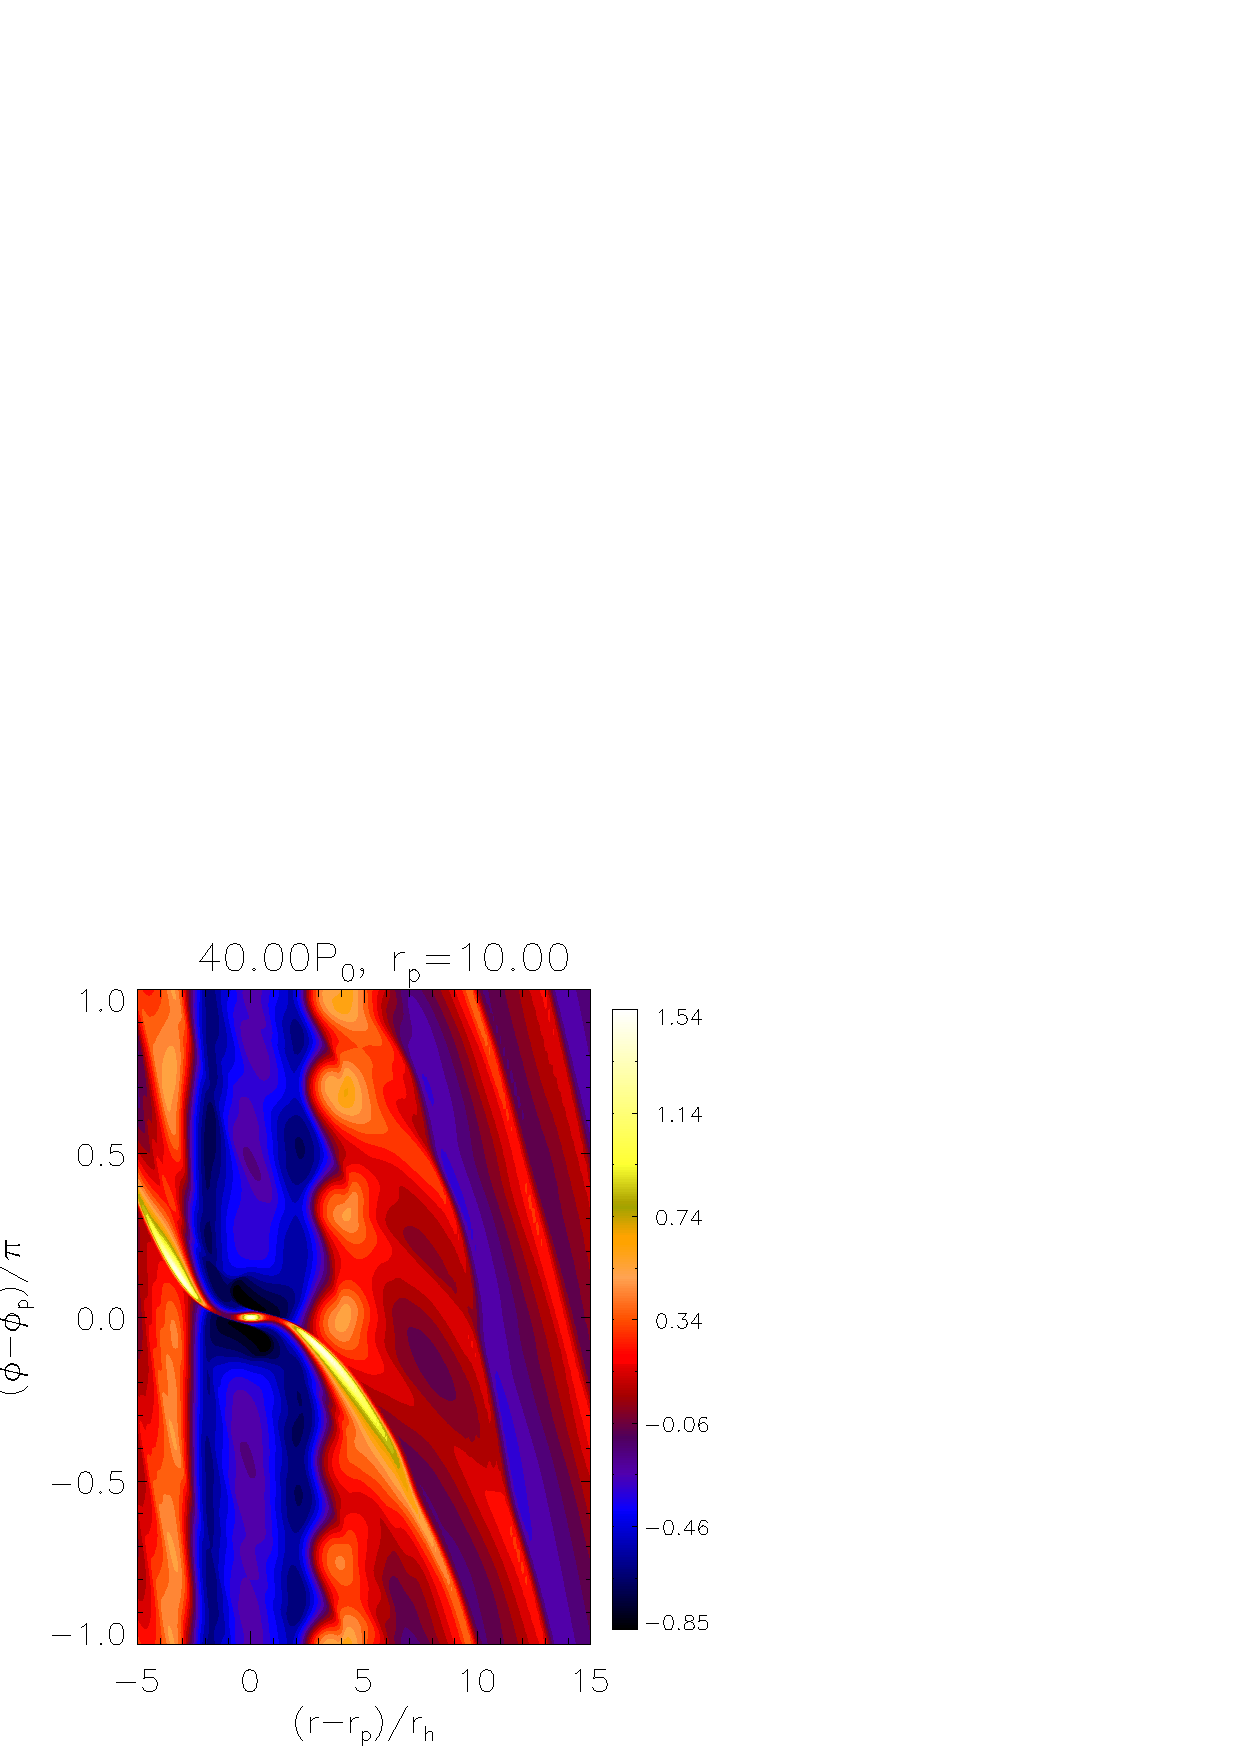
\includegraphics[scale=.55,clip=true,trim=2.26cm 0cm 0cm
%% %    0cm]{figures/noniso1_HR_dens004}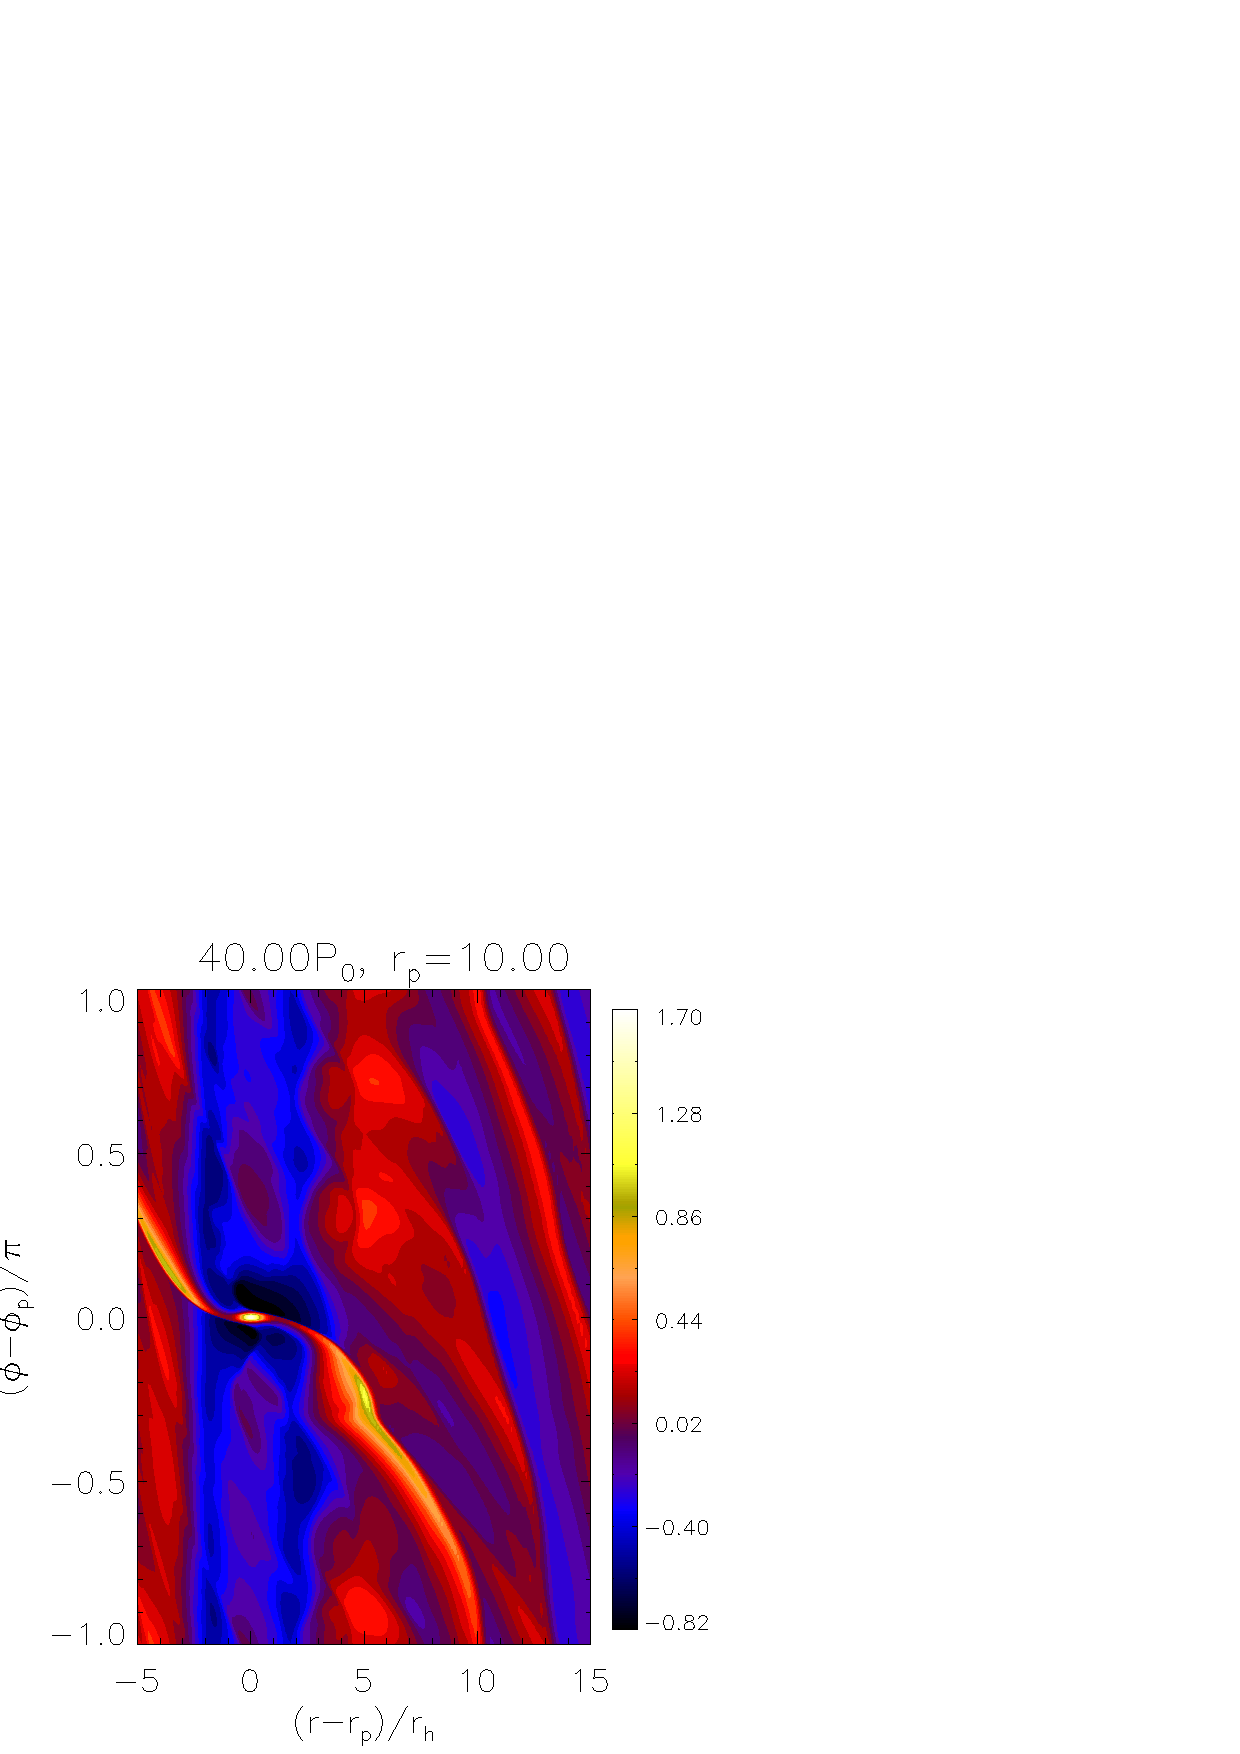
\includegraphics[scale=.55,clip=true,trim=2.26cm 0cm 0cm
%% %    0cm]{figures/noniso2_HR_dens004}
%%   \caption{Gap instability in the heavy disc model, as a function of
%%     the cooling parameter: $\tbeta=0.1$ (left), $\tbeta=1$ (middle)
%%     and $\tbeta=10$ (right). The relative surface density
%%     perturbation is shown. \label{polarxy_q1d5}} 
%% \end{figure*}

%\input{discussion}
%\section{Summary and discussion}\label{summary}
In this paper, we have carried out numerical simulations of non-isothermal disc-planet interaction. 
Our simulations were customised to examine the effect of a finite cooling time on the stability of gaps 
opened by giant planets to the so-called vortex or Rossby wave instability. To do so, we 
included an energy equation with a cooling term that restores the initial disc temperature on a characteristic timescale $t_c$. 
We studied the evolution of the gap stability as a function of $t_c$. This is a natural extension to previous
studies of on gap stability, which employ locally or strictly isothermal equations of state. 	

We considered two types of numerical experiments. 
We first used disc-planet interaction to self-consistently set up
gap profiles, which were then perturbed and evolved without further the influence of the planet potential. This procedure  
isolates the effect of cooling on gap stability through the set up of the initial gap profile. We find that as the cooling time $t_c$ is increased,
the gaps became more stable, with lower growth rates of non-axisymmetric modes and the dominant azimuthal wavenumber also decreases. 
This is consistent with the notion that increasing $t_c$ leads to higher temperatures or $h$, which opposes gap-opening by the planet. This means that
the gaps opened by the planet in a disc with longer $t_c$ is smoother and therefore  more stable to the RWI. 


In the second set of calculations, we included the planet potential throughout the simulations 
and examined the long-term evolution of the gap-edge vortex that develops from the RWI. The vortices to reach a
quasi-steady state lasting $O(10^3)$ orbits, during which its amplitude grows until it begins to induce shocks,  
afterwhich the vortex amplitudes decay. 
We observe vortex lifetimes to increase with increasing cooling time until
a cooling timescale on the order of the libration time at the gap edge {\bf (this statement assumes longest lifetime is $\tilde{\beta}=1$, so may change
depending on new definitions of lifetimes)}, beyond which vortex lifetimes shorten again. 

Our results indicate there exists an optimum cooling timescale to maximise the lifetime of gap-edge vortices. We suggest the non-monotonic dependence
can be attributed to the time required for the vortex to grow to sufficient amplitude to induce shocks in the surrounding fluid, thereby losing energy and also smooth out the gap edge.  
For short cooling timescales, the planet is able to open a deeper gap which favours the RWI, leading to stronger vortices. However, for long 
cooling timescales, the vortex grow faster during the quasi-steady state {\bf check if statement true}. 
We suggest the latter is due to the RWI being favoured with increasing disc temperature, according to previous stability
calculations. These competing factors imply for both very short and long cooling timescales, the vortex reaches its maximum amplitude 
, shocks, and begins to decay, sooner than intermediate cooling timescales. 
%decay timescale depends on cooling time, but there seems to be a monotonic trend: longer cooling times, decay timescale is shorter, so this 
%doesn't contribute to non-monotonic part

We remark that a non-monotonic dependence of the vortex lifetime was also reported
by \cite{fu14}, who performed isothermal disc-planet simluations with different values of the 
disc aspect ratio. In their simulations the optimum aspect ratio is $h=0.06$. In our simulations,
the aspect ratio is a dynamical variable, but by analysing the region where the vortex is located ($r-r_p\in[2,10]r_h$), 
% {\bf define this region}
we find for $\tilde\beta=5.0$ case, with the longest vortex lifetime, has
$h\approx0.06$ on average throughout its lifetime. 
{\bf if new definition of vortex lifetime gives other $\tilde{\beta}$ values as the maximum lifetime, then need to update this value of $h$}. 
Our result is therefore qualitatively consistent with \citep{fu14}. 
%This value of $h$ was also
%found to maximise vortex lifetimes in the simulations of
%\cite{fu14}. Note that $h$ is a fixed parameter in \cite{fu14} while in
%our simulations $h$ is a dynamical variable. 

\subsection{Caveats and outlooks}
We discuss below several outstanding issues that needs to be addressed in future works:

\emph{Convergence.} Although lower-resolution simulations performed in the early stages of this project gave similar results 
(most importantly, the non-monotonic dependence of vortex lifetimes on the cooling timescale), we did find the lower-resolution simulations 
typically yield longer vortex lifetimes than that reported in this paper. This could be due to weaker RWI with low resolution. 
It will be neccessary to perform even higher resolution  simulations in order to obtain quantitatively converged vortex lifetimes. 
 
\emph{Self-gravity.} We have ignored disc self-gravity in this study. Based on linear calculations, \cite{lovelace13} concluded self-gravity
to be important for the RWI when $Q<O(1/h)$, or $Q\lesssim 20$ for $h\sim0.05$, as was typially considered in this work. This suggests that 
self-gravity may affect vortex lifetimes even when the Toomre $Q$ parameter is not small. In particular, given that we observe
vortices can reach significant over-densities (up to almost an order of magnitude), it will be important to include disc self-gravity 
in the future. %self-gravitational collapse of vortices 
 
\emph{Three-dimensional (3D) effects.} A vortex in a 3D disc may be subject to secondary instabilities 
that destroy them \citep{lesur09,railton14}. This may an important factor in determining gap-edge vortex lifetimes
in realistic discs. For example, if these secondary instabilities sets in before the vortex grows to sufficient amplitude to shock, 
then the dependence of the vortex lifetime on the cooling timescale will be that through the 3D instability (as opposed to the effect on the RWI itself).  
This problem needs to be clarified with full 3D disc-planet simulations. 

%3d is challenging because high resolution needed in for 3d instabilities
%However, the role of these instabilities on gap-edge vortices, where disc-planet  
%interaction can maintain the RWI, has not been clarified.  


%\section*{Acknowledgments}

\bibliographystyle{mn2e}
\bibliography{ref}

\appendix
%\input{appendix}
%\input{appendix2}

\end{document}
